Facial analysis in images for recognition/manipulation is a widely addressed and commercially important problem. 
Its applications range from surveillance to automatic tagging of photos on social websites. 
Recently, there are papers producing convincing results on {\em in-the-wild}
datasets~\cite{Ramanan:2012:FDP:2354409.2355119,DBLP:journals/corr/HassnerHPE14}. These
datasets differ from previous ones in their unconstrained nature of image capture.
However such methods have two drawbacks. Firstly, a lot of these methods have degraded performance in profile view vs frontal view. 
Secondly, they require lot of training data~\cite{HuLT14}. One way to alleviate both problems is to be able 
to generate realistic frontal view faces for any person. This can be achieved, because faces have a definite 
structure. Eigen analysis~\cite{Belhumeur:1997:EVF:261506.261512}, for example, has shown that faces exist in low dimensional sub spaces and can be represented as linear combinations of other faces. Also, it has been shown earlier that many face characteristics like expressions, hair etc. can be \emph{transferred} from one person to another, in a very realistic manner~\cite{conf/fgr/SaragihLC11a}.

\begin{figure}
\begin{center}\includegraphics[width=11.0cm,height=2.8cm]{front/figures/sample_result_f.png}\end{center}
\caption{Left image shows the profile face. Second image is {\em face frontalized} by our method. Third image is of Hassner {\em et al.}~\cite{DBLP:journals/corr/HassnerHPE14} method. Right image is the natural frontal view of the individual. {\em Frontalization} helps in face recognition. }
\label{fig:sample_result}
\end{figure}

In this paper, we show that a pre-processing step of synthesizing frontal pose of the face
significantly improves the accuracy of face recognition. Face frontalization is the process of
synthesizing frontal pose of the face, given a profile view of the face as shown in
Figure~\ref{fig:sample_result}. This step helps in simplifying the task of face recognition as
recognition systems have more information and less occlusion to work with. Few methods counter this
{\em frontalization} problem, by choosing to extract features only at the salient locations.
Unfortunately, this leads to loss of structural relation between various parts of the face. However,
as we will show in this paper, our method preserves this information as well. 

Apart from aiding face recognition systems, frontalization techniques can also be used to generate a video out of a single image 
and can find applications in animation~\cite{conf/fgr/SaragihLC11a}. For example, if a family photograph has some people 
looking away from the camera, our approach can be used to correct this discrepancy~\cite{Oh:2001:IMP:383259.383310}. 

Recent methods~\cite{SunWT14}~\cite{surpassing_human} have proposed different ways of addressing the
challenging problems of pose variations in images. Simonyan {\em et al.}~\cite{surpassing_human}~\cite{simonyan13fisher}
choose to define features extracted out of large image regions to counter
mis-alignments. Wolf {\em et al.}~\cite{HuangJL07}~\cite{Wolf} choose to align faces before extracting
features. Sun {\em et al.}~\cite{HuLT14} use large datasets to create models robust to these
challenges. In line with our approach, some recent works try to counter these challenging conditions of pose variation by
synthesizing pose neutral faces from input images. Taigman {\em et al.}~\cite{Taigman_2014_CVPR}
try to estimate a {\sc 3d} model of each input image. They then  use this {\sc 3d} information to synthesize
the frontal view. On the other hand, ~\cite{DBLP:journals/corr/HassnerHPE14} assumes a generic {\sc 3d} model for
all input images and produces convincing frontalization results. Even though the approach of~\cite{Taigman_2014_CVPR} seems to be good, estimating {\sc 3d} model from a single image is a hard problem. And assuming a generic {\sc 3d} model in~\cite{DBLP:journals/corr/HassnerHPE14}, leads to loss of structural information unique to an individual.
 Thus, in this work, we turn towards an exemplar based approach to fill the {\sc 3D} information gap 
required by the previous approaches. 
% \begin{figure}
% \begin{center}\includegraphics[width=9.0cm,height=2.8cm]{../images/sample_result_f.png}\end{center}
% \caption{Left image shows the profile face. Second image is {\em face frontalized} by our method. Third image is of Hassner {\em et al.}~\cite{DBLP:journals/corr/HassnerHPE14} method. Right image is the natural frontal view of the individual. {\em Frontalization} helps in face recognition. }
% \label{fig:sample_result}
% \end{figure}
% \begin{figure*}
% 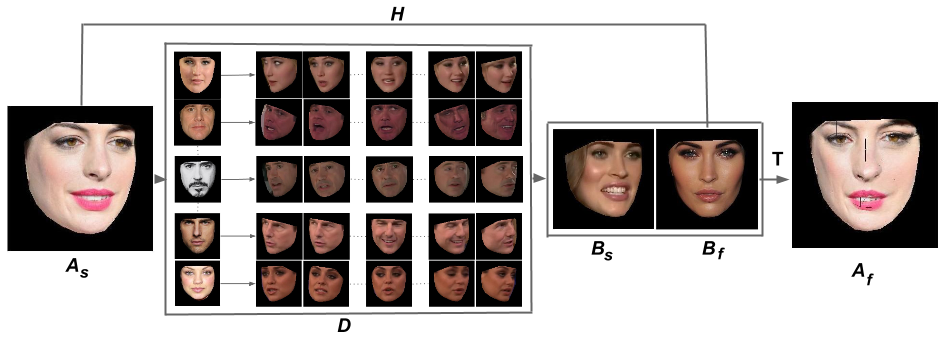
\includegraphics[width =18cm,height=6.6cm]{../images/Method_Pipeline.png}
% \caption{Figure shows the generic pipeline used in our approach. Given the input image (left most
% block) we use the exemplar database (second block) to compute the nearest profile view (third block,
% first image). We then use the correspondences between the profile and frontal views of the
% selected exemplar pair (third block) to compute the affine transformation $H$ between the input
% image and the frontal exemplar, and use it to produce the \emph{frontalized output} (right most block).}
% \label{fig:method_pipeline}
% \end{figure*}

Lately, we have seen a surge of papers~\cite{malisiewicz-iccv11}~\cite{B-WeiBoy08} based on exemplar methods for solving computer vision problems. 
In these type of approaches, exemplars of the problem category are used instead of defining a
generic model to solve the 
the problem at hand. For example, in the case of object detection,~\cite{malisiewicz-iccv11} trains a set of models 
using one positive exemplar each, instead of all the training set. And they show that the ensemble of such 
models give surprisingly good generalization. Similarly, our method is based on an exemplar based approach 
toward face frontalization. Consider a huge dataset of profile, frontal view face pairs of different. Chances of finding 
individuals with similar face structures to an input profile image is thus very high. Given such a
match, the frontal view of the person in the database can then be used to frontalize the input
image.  Therefore, for our method, we collect a database 
of profile views and corresponding frontal view of a large number of individuals. We leverage the fact that 
faces lie in a low dimensional subspace and thus, many characteristics, like pose, expressions, etc.
are transferable between people.
